\chapter{Data Preparation}

\begin{figure}[hbtp]
	\centering
	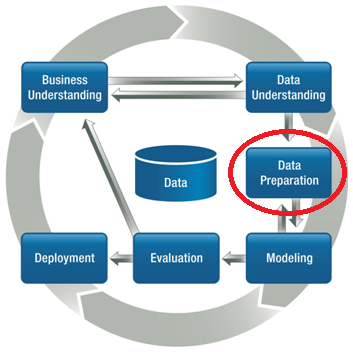
\includegraphics[width=0.5\textwidth]{./images/CRISPDM_3.png}
	\caption{CRISP-DM - Data Preparation}
	\label{CRISPDM_3}
\end{figure}



\section{Criteri di Inclusione/Esclusione dei dati}


\section{Selezione dei dati}

\section{Campionamento}


\section{Feature Selection}
By Rino:
Per questi scopi, WEKA fornisce l'operatore CfsSubsetEval il quale valuta il "worth" del subset di attributi considerando la singola correlazione di ognuno con l'attributo di classe. La ricerca nello spazio del subset degli attributi può essere realizzato essenzialmente attraverso la strategia best first la quale cerca by greedy hillclimbing augmented with a backtracking facility.
La best first may start with the empty set of attributes and search forward, or start with the full set of attributes and search backward, or start at any point and search in both directions.

By Weka:
Evaluates the worth of a subset of attributes by considering the individual predictive ability of each feature along with the degree of redundancy between them.
NAME
weka.attributeSelection.CfsSubsetEval

SYNOPSIS
CfsSubsetEval :

Evaluates the worth of a subset of attributes by considering the individual predictive ability of each feature along with the degree of redundancy between them.

Subsets of features that are highly correlated with the class while having low intercorrelation are preferred.

For more information see:

M. A. Hall (1998). Correlation-based Feature Subset Selection for Machine Learning. Hamilton, New Zealand.



By Wiki:
CFS Feature Set Evaluation

CFS is a correlation-based filter method CFS from [Hal98]. It gives high scores to subsets that include features
that are highly correlated to the class attribute but have low correlation to each other Let S be an attribute
subset that has k attributes, rcf models the correlation of the attributes to the class attribute, rff the
intercorrelation between attributes.


NAME
weka.attributeSelection.BestFirst

SYNOPSIS
BestFirst:

Searches the space of attribute subsets by greedy hillclimbing augmented with a backtracking facility. Setting the number of consecutive non-improving nodes allowed controls the level of backtracking done. Best first may start with the empty set of attributes and search forward, or start with the full set of attributes and search backward, or start at any point and search in both directions (by considering all possible single attribute additions and deletions at a given point).


OPTIONS
direction -- Set the direction of the search.

lookupCacheSize -- Set the maximum size of the lookup cache of evaluated subsets. This is expressed as a multiplier of the number of attributes in the data set. (default = 1).

searchTermination -- Set the amount of backtracking. Specify the number of 

startSet -- Set the start point for the search. This is specified as a comma seperated list off attribute indexes starting at 1. It can include ranges. Eg. 1,2,5-9,17.

\section{Data Cleaning}

\section{Construct Data}

\section{Integrate Data}

\section{Format Data}
Format ARFF
